\chapter{真实世界坐标系下的地图生成与定位方法设计}
\label{cha:chap2}

\section{引言}
\label{sec:2.1}
基于SLAM方法的即时建图和定位方法目前已经发展到的相当成熟,尤其是在无人机、无人车领域,基于视觉SLAM方法进行定位有着积
极地应用,对于实际落地的场景,该系统输出的相机位姿和构建的地图必须具备真实尺度才能够进行导航与定位,此外依靠视觉构建
的地图所处坐标系往往取决于初始化成功后的第一帧多建立的坐标系,这些问题的存在都使得传统SLAM系统难以有实际的使用条件。

对于当前传统的单目视觉SLAM算法,设备简易,处理数据较少,满足实时性的要求,但是也存在只能获取相机坐标系下得到相机位姿
以及无法获取地图实际尺度的问题,无法展开实际应用;对于基于双目视觉的SLAM算法,可以解决地图尺度的问题,但面临成本较高,
相机标定难度大且精度不高,鲁棒性较差等问题;对于融合视觉和IMU传感器的SLAM系统,可以获取真实尺度,以及得到真实世界坐
标系下的相机和地图位姿,但是该系统对于IMU的精度要求较高,且在引入IMU后容易产生累计误差,难以初始化成功等问题。

针对上述问题,本章提出一种融合视觉传感器和二维码标签的单目视觉SLAM方法,在传统SLAM功能的基础上,可以得到相机和地图的
真实尺度,并且根据一定的坐标转换,可以得到真实世界坐标系下的相机位姿和地图。在真实的应用场景中,布置的二维码和普通的自
然特征点相比,更加容易捕捉到特征点,此外,比较固定,在重定位的流程中,往往会有更好的效果。该系统能够具备以下优良特性:
能够对地图进行保存,复用和更新,通过不断完善的先验地图提高系统的鲁棒性;添加二维码信息增强传统SLAM中的重定位问题,此
外通过二维码的尺度在仅适用单目相机的情况下估算出真实地图的尺度;依靠二维码中坐标系和真实世界的坐标系的转化,获取待估计
物体在真实世界下的位姿。本章所提出来的结合二维码的视觉SLAM算法流程如图2.1所示,主要过程包括二维码。
\section{二维码检测与识别方法}
\label{sec:2.2}
\subsection{二维码检测与识别方法}
\label{sec:2.2.1}
二维码和一般的自然特征点相比较,具备比周围环境亮度更低得到的显著特点,如图~\ref{fig:Aruco_Aruco_Gradient}所示;且
二维码本身是一个四边形的区域,可以凭借该特点约束出后续相机的位姿的绝对尺度;并且每一个二维码通过解码都可以获取到一个
独一无二的对应ID号序号,在SLAM重定位的过程中,可以避免高重合区域的误检,在通过视觉检测二维码得到的过程中,我们希望尽
可能多的检出场景中的所有二维码,随后再通过编码对误检值进行剔除。
\begin{figure}[H]
  \centering%
  \subcaptionbox{ArUco二维码原始图像\label{fig:Aruco}}{%    
    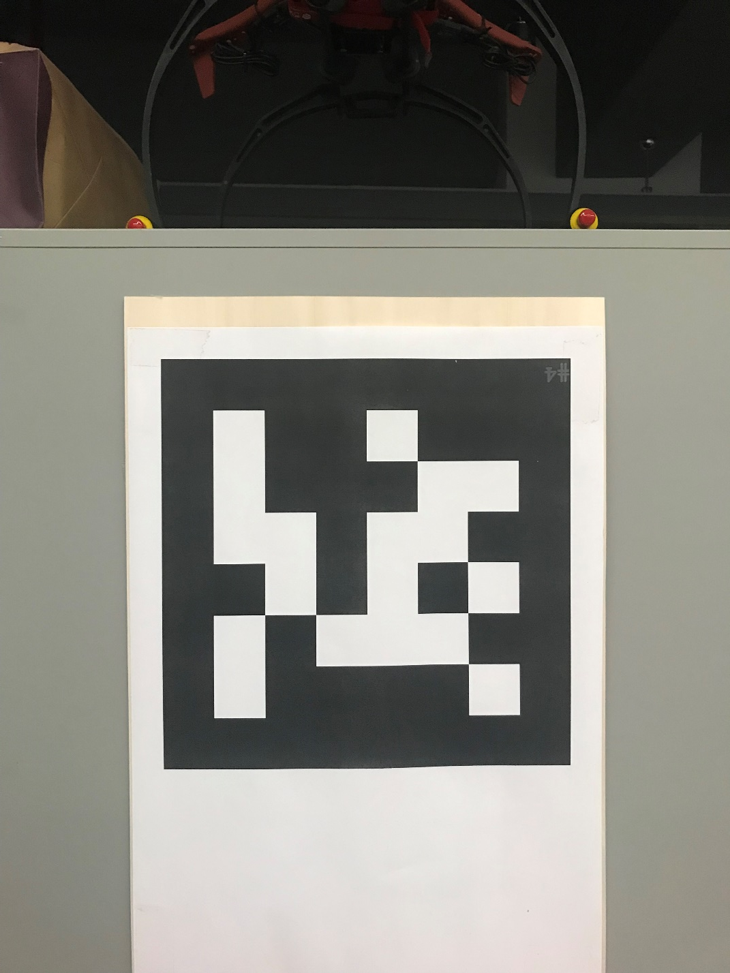
\includegraphics[height=5cm]{Aruco.png}}\hspace{4em}%
  \subcaptionbox{ArUco二维码原始图像\label{fig:Aruco_Gradient}}{%    
    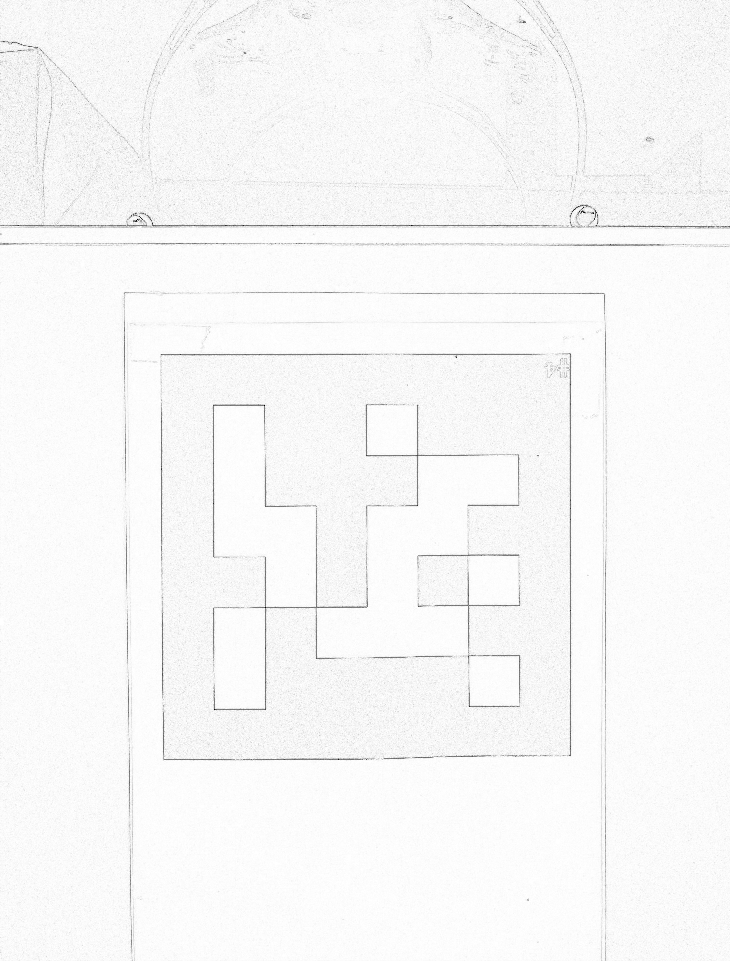
\includegraphics[height=5cm]{Aruco_Gradient.png}}
  \caption{ArUco二维码原始图像和梯度图}
  \label{fig:Aruco_Aruco_Gradient}
\end{figure}

\subsection{ArUco二维码的检测和识别过程}
\label{sec:2.2.2}
ArUco的检测和识别过程主要包括检测出二维码4个角点在图像中的位置,以及被检出的二维码的ID序号,在检测4个角点的位置时,
需要检测图像中的线段和构成二维码的四边形。

在线段检测阶段,首先会计算整个图片中每一个像素的梯度强度大小和方向,随后对计算所得的梯度进行聚类,对所有满足聚类条
件的像素点进行合并,可以的得到一组连续点,即检测出线段。

检测完线段后,进一步的需要检测构成二维码边缘的四边形,针对上一步中获取到的所有线段,对线段进行分组,若满足,上一线
段的末端点和下一线段的起始点之间的距离小于某一阈值,即可首尾进行按照逆时针进行连接,若所有连接的线段数量达到4时,即
认定生成的闭环可能为一个二维码的边缘四边形。

在检测二维码ID值之前,会先设定好一个包含所有二维码的字典,字典的大小即二维码的数量,字典中元素的大小即是每一个二维
码的位数量。检测出构成二维码的四边形后,需要对图像进行透视变化规范图像,随后通过设定阈值分离出二维码上的黑色位和白
色位,通过位数情况即可判断该二维码是否是字典外的不合规值,以及字典中的特定ID值,识别结果如图~\ref{fig:Aruco_detection}所示。通过这样的方式
检测和识别二维码具备非常好的鲁棒性,并且可以对错误值进行效验。
\begin{figure}[H] % use float package if you want it here
  \centering
  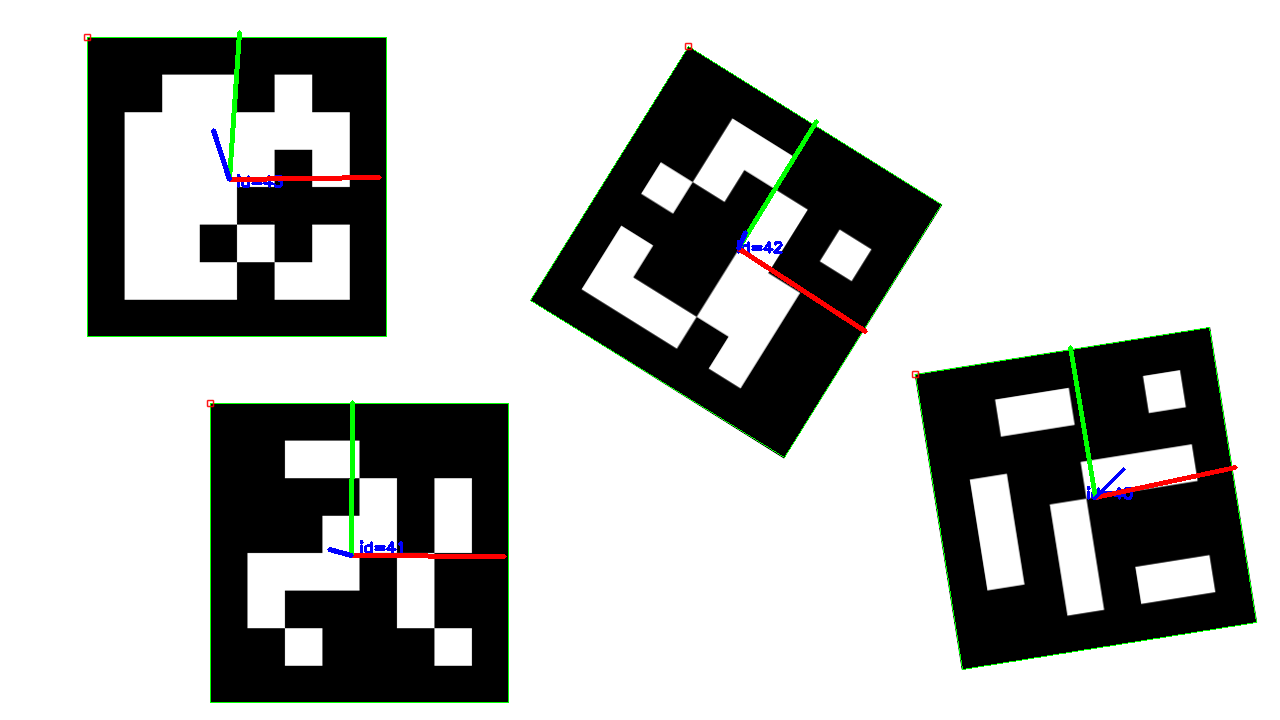
\includegraphics[height=8cm]{Aruco_detection.png}
  \caption{ArUco二维码识别结果示意图}
  \label{fig:Aruco_detection}
\end{figure}

\subsection{估计相机外参}
\label{sec:2.2.3}
对于传入的单帧图像,在提取完二维码的四边形轮廓,4个角点以及检测对应的唯一ID值后,接下来会估计检出的二维码位姿,包括
平移向量和旋转向量,相机的外参主要是通过PnP方法,利用4对点来求解。

为了简化定位的过程,以二维码的坐标系作为世界坐标系,二维码边长为S,则四个角点的坐标分别为A(-S/2,S/2,0),
B(S/2,S/2,0),C(S/2,-S/2,0),D(-S/2,-S/2,0),在图像中的对应像素点为a(u_a,v_a), b(u_b,v_b),
 c(u_c,v_c), d(u_d,v_d)。因为相机的内参K提前标定,则三维空间中的点和像素坐标中的点之间的转换关系可以表示为:


\section{图的例子}
\label{sec:other}

在第~\ref{cha:intro} 章中我们学习了贝叶斯公式~(\ref{equ:chap1:bayes}),这里我们复
习一下:
\begin{equation}
\label{equ:chap2:bayes}
p(y|\mathbf{x}) = \frac{p(\mathbf{x},y)}{p(\mathbf{x})}=
\frac{p(\mathbf{x}|y)p(y)}{p(\mathbf{x})}
\end{equation}

\subsection{绘图}
\label{sec:draw}

本模板不再预先装载任何绘图包(如 \textsf{pstricks,pgf} 等),完全由你自己来决定。
个人觉得 \textsf{pgf} 不错,不依赖于 Postscript。此外还有很多针对 \LaTeX{} 的
 GUI 作图工具,如 XFig(jFig), WinFig, Tpx, Ipe, Dia, Inkscape, LaTeXPiX,
jPicEdt, jaxdraw 等等。

\subsection{插图}
\label{sec:graphs}
关于子图形的使用细节请参看 \textsf{subcaption} 的说明文档。

\subsection{一个图形}
\label{sec:onefig}
一般图形都是处在浮动环境中。之所以称为浮动是指最终排版效果图形的位置不一定与源文
件中的位置对应\footnote{This is not a bug, but a feature of
\LaTeX!},这也是刚使 用 \LaTeX{}
同学可能遇到的问题。如果要强制固定浮动图形的位置,请使用
\textsf{float} 宏包, 它提供了 \texttt{[H]}
参数,比如图~\ref{fig:heythere}。
\begin{figure}[H] % use float package if you want it here
  \centering
  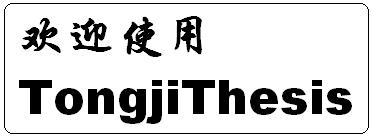
\includegraphics[height=2cm]{hello.jpg}
  \caption{插个图插个图}
  \label{fig:heythere}
\end{figure}

大学之道,在明明德,在亲民,在止于至善。知止而后有定;定而后能静;静而后能安;安
而后能虑;虑而后能得。物有本末,事有终始。知所先后,则近道矣。古之欲明明德于

\hfill \pozhehao《大学》


\subsection{简单子图}
\label{sec:multifig}

如果多个图形相互独立,并不共用一个图形计数器,那么用 \verb|minipage| 或者
\verb|parbox| 就可以。否则,请参看图~\ref{fig:big1},它包含两个小图,分别是图~\ref{fig:subfig1}
和图~\ref{fig:subfig2}。推荐使用 \verb|\subcaption|,不要再用\verb|\subfloat|,\verb|\subfigure| 和 \verb|\subtable|了。
\begin{figure} %[h]
  \centering%
  \subcaptionbox{第一个小图形\label{fig:subfig1}}{%    
    
\includegraphics[height=2cm]{tongji-fig-logo.png}}\hspace{4em}%
  \subcaptionbox{第二个小图形。如果标题很长的话,它会自动换行,这个 caption 就是这样的例子\label{fig:subfig2}}{%    
    
\includegraphics[height=2cm]{tongji-text-logo.png}}
  \caption{包含子图形的大图形}
  \label{fig:big1}
\end{figure}

古之学者必有师。师者,所以传道受业解惑也。人非生而知之者,孰能无惑?惑而不从师,
其为惑也,终不解矣。生乎吾前,其闻道也固先乎吾,吾从而师之;生乎吾後,其闻道也亦
先乎吾,吾从而师之。吾师道也,夫庸知其年之先後生於吾乎!是故无贵无贱无长无少,道
之所存,师之所存也。

嗟乎!师道之不传也久矣,欲人之无惑也难矣。古之圣人,其出人也远矣,犹且从师而问焉;
今之众人,其下圣人也亦远矣,而耻学於师。是故圣益圣,愚益愚。圣人之所以为圣,愚


\subsection{复杂子图要注意遮挡}
使用子图的方法如图~\ref{fig:chap2:zitu}所示,使用\texttt{subcaptionbox}环境设置每一个子图,注意\texttt{subcaptionbox}其后需要有括号,以及子图换行时需要使用\texttt{vskip},以免下一排子图会对上一排子图的图名造成遮挡。
\begin{figure}[htbp]
\centering
  \subcaptionbox{第一个小图形}{\label{fig:chap1:zitu:a}
  
\includegraphics[width=5cm]{tongji-fig-logo}\hskip2cm}
  \subcaptionbox{第二个小图形}{\label{fig:chap1:zitu:b}
  
\includegraphics[width=5cm]{tongji-fig-logo}}
\vskip0.5cm
  \subcaptionbox{第三个小图形}{\label{fig:chap1:zitu:c}
  
\includegraphics[width=5cm]{tongji-fig-logo}\hskip2cm}
  \subcaptionbox{第四个小图形}{\label{fig:chap1:zitu:d}
  
\includegraphics[width=5cm]{tongji-fig-logo}}
\caption{多子图用\texttt{subcaptionbox}}\label{fig:chap2:zitu}
\end{figure}


\subsection{多个图形独立}
如果要把编号的两个图形并排,那么小页就非常有用了,如图~\ref{fig:parallel2}:
\begin{figure}
\begin{minipage}{0.48\textwidth}
  \centering
  
\includegraphics[height=2cm]{tongji-whole-logo.png}
  \caption{并排第一个图}
  \label{fig:parallel1}
\end{minipage}\hfill
\begin{minipage}{0.48\textwidth}
  \centering
  
\includegraphics[height=2cm]{tongji-whole-logo.png}
  \caption{并排第二个图}
  \label{fig:parallel2}
\end{minipage}
\end{figure}


李氏子蟠,年十七,好古文、六艺,经传皆通习之,不拘於时,学於余。余嘉其能行古
道,作师说以贻之。

\hfill \pozhehao 韩愈(唐)


\subsection{插图大原则}
同志们,如果遇到问题一定要会搜索,要么看别人的问答,要么看宏包的文档,希望你不要成为重度伸手党。
一点微小的工作,谢谢大家。

\section{插入pdf格式图片的问题}
\label{sec:problem}
在\LaTeX{}中插入高清图片一般有两种方式:1)插入~eps~矢量图,2)插入~pdf~格式图片。在模板测试过程中遇到一个插入
~pdf~格式图片的问题。

问题描述

插入~pdf~格式的图,有时采用~XeLaTeX~编译后,插图被翻转~90~度。有时却不会出现该问题。问题图片如图~\ref{rotatedBode}~所示。
\begin{figure}[H] 
  \centering
  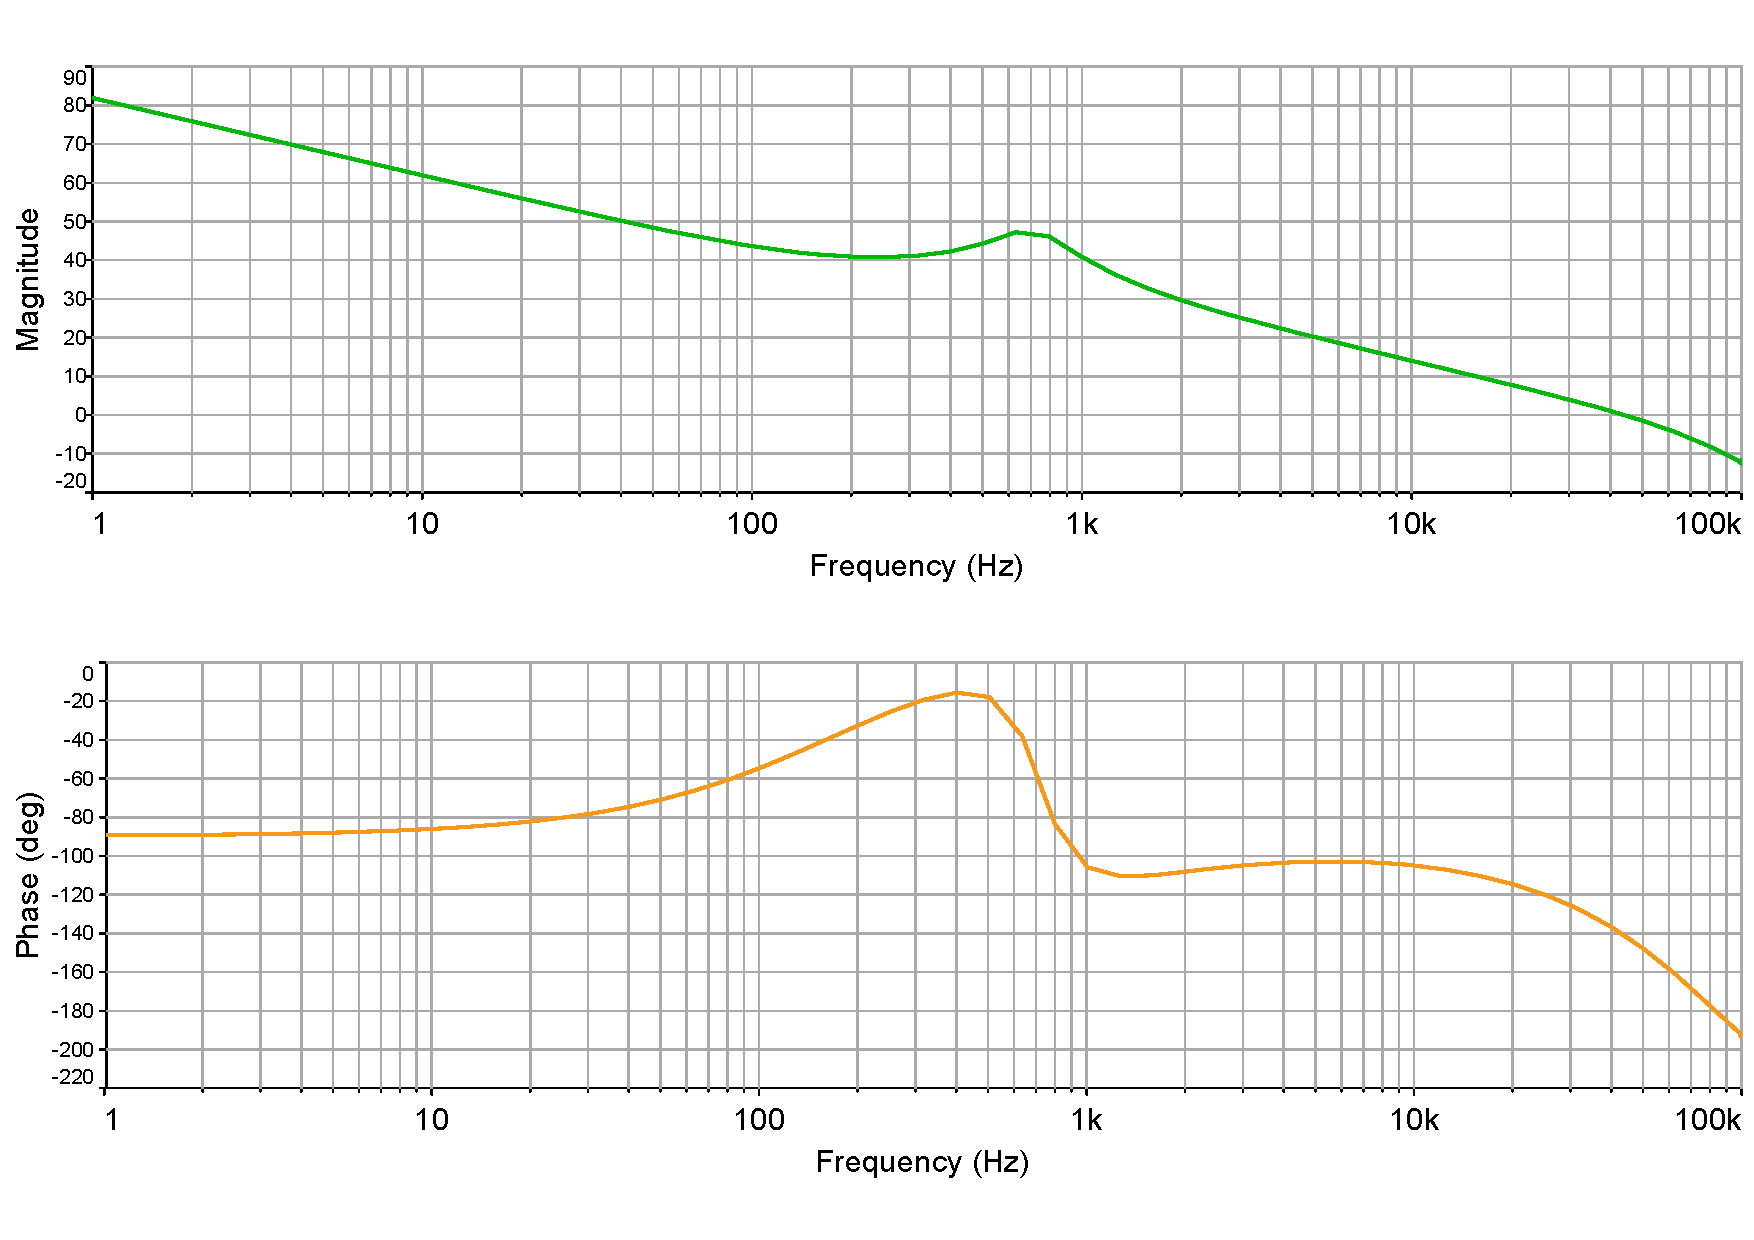
\includegraphics[width=12cm]{BodeGraph.pdf}
  \caption{被自动翻转的bode图}
  \label{rotatedBode}
\end{figure}

问题原因

同一幅图片,XeLaTeX~编译出现图片翻转,而~pdfLaTeX~编译,输出正常。
原因可能是出现在~XeLaTeX~编译过程中会将有些~pdf~文件自身多余的旋转命令编译出来。

问题解决方法

第一种方法(抄自刘海洋大牛的方案):
使用命令\\ \texttt{pdfcrop foo.pdf foo-new.pdf},当然,新文件名可以和旧文件名相同。 这个方法的好处就是 pdfcrop 是texlive自带的,我装的是texlive2017,因此自带了。

第二种方法:采用GhostScript软件消除多余的旋转命令。
\begin{enumerate}
    \item 下载安装~GhostScript~软件,官网为\url{https://www.ghostscript.com/download/gsdnld.html/}
        
    \item 将安装后的bin文件夹地址加入用户环境变量,在我电脑上为~\verb|D:|\verb|\Program Files|\verb|\gs|\verb|\gs9.22|\verb|\bin|
	
    \item cmd~命令行进入想转换图片所在文件夹,执行命令\\gswin32c -sDEVICE=pdfwrite -o newname.pdf  previousname.pdf
              得到一个去除多余旋转命令的~newname.pdf~文件。

    \item 在\LaTeX{}中插入该~pdf~文件,XeLaTeX~编译。
\end{enumerate}

处理之后的图片如图~\ref{Bode}~所示。
\begin{figure}[H] 
  \centering
  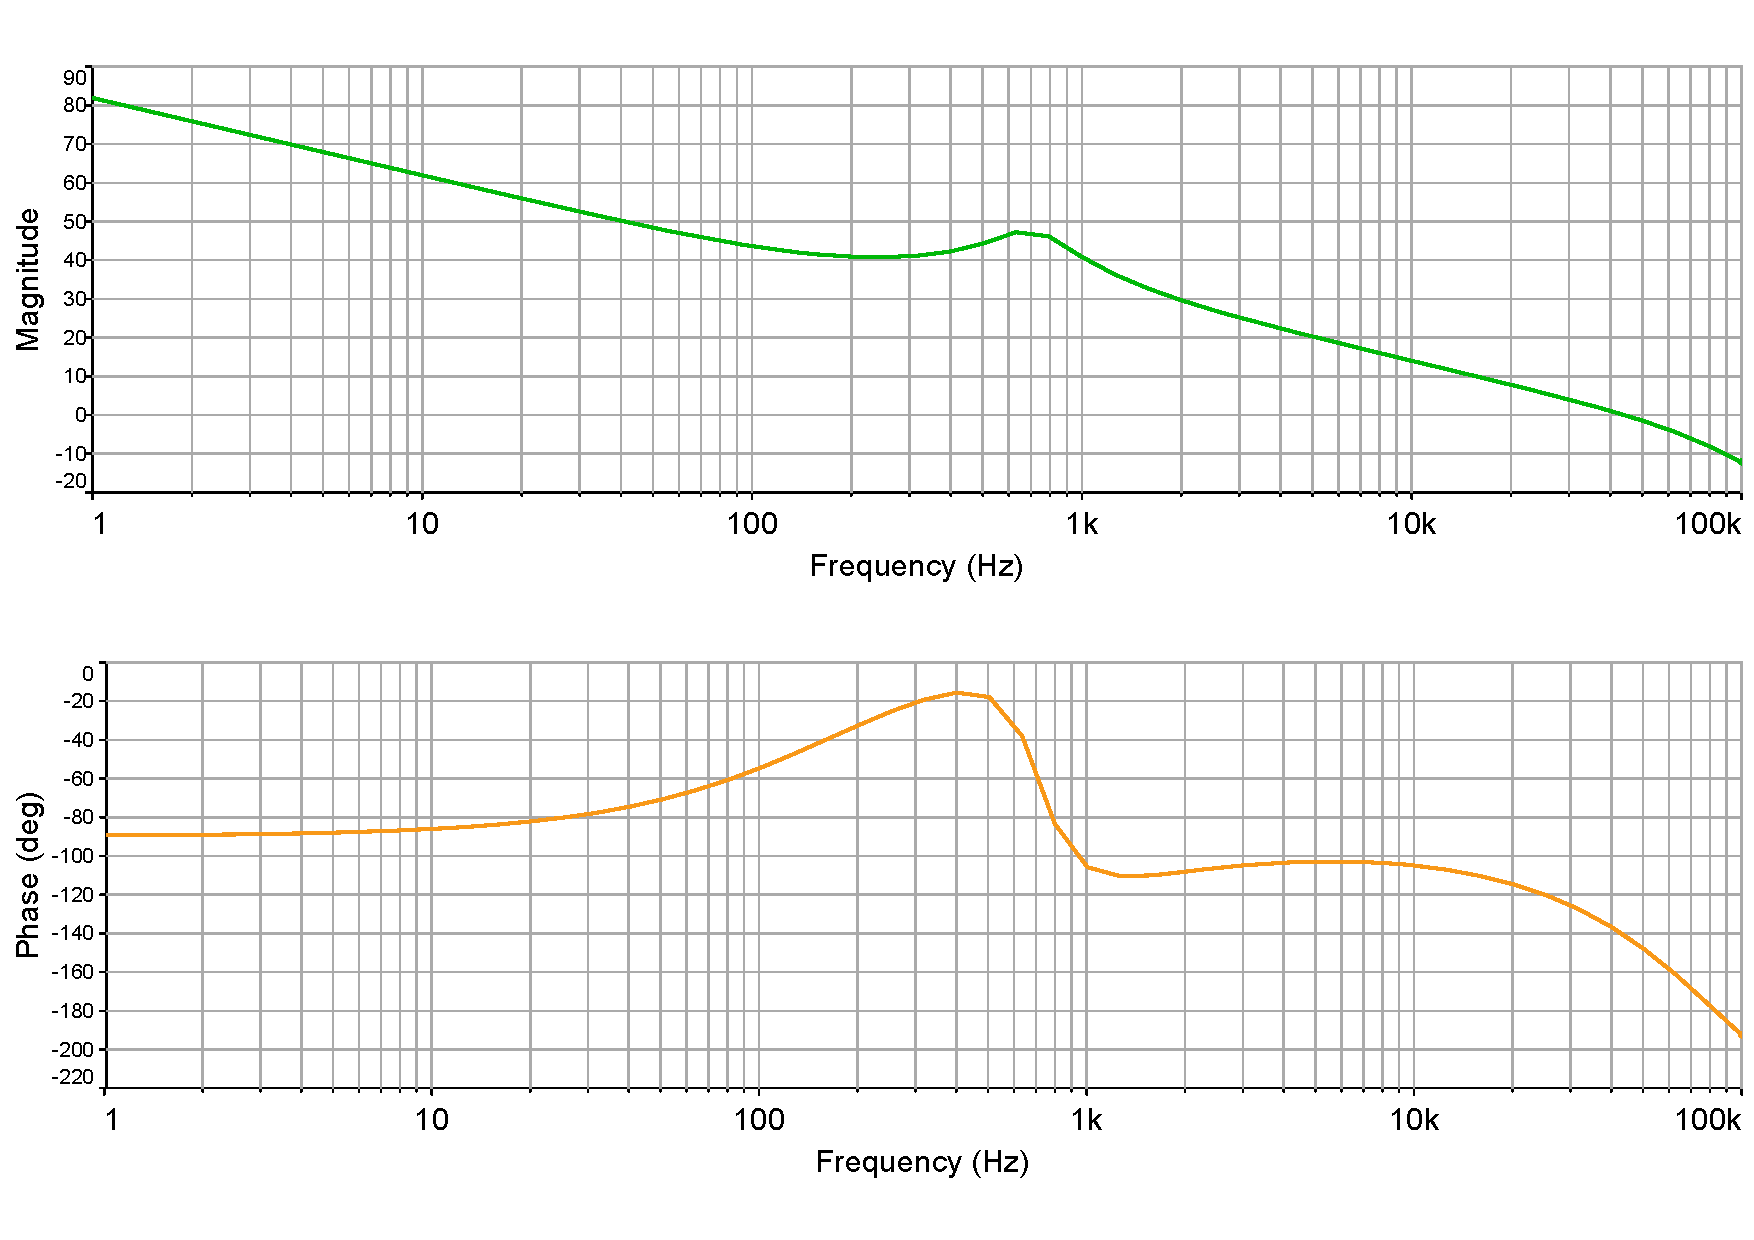
\includegraphics[width=12cm]{Bode.pdf}
  \caption{处理后的bode图}
  \label{Bode}
\end{figure}





